%%________________________________________________________________________
%% LEIM | PROJETO
%% 2022 / 2013 / 2012
%% Modelo para relatório
%% v04: alteração ADEETC para DEETC; outros ajustes
%% v03: correção de gralhas
%% v02: inclui anexo sobre utilização sistema controlo de versões
%% v01: original
%% PTS / MAR.2022 / MAI.2013 / 23.MAI.2012 (construído)
%%________________________________________________________________________




%%________________________________________________________________________
\chapter{Introdução}
\label{ch:introducao}
%%________________________________________________________________________

Este trabalho teórico-prático tem como objetivo: na primeira parte, desenvolver um modelo ontológico a partir de conceitos teóricos definidos em documentos oficiais da DGS no contexto da pandemia.

Na segunda parte, procedeu-se à resolução do caderno de exercícios sobre Lógica de Descrição, consolidando os fundamentos teóricos que estão como foco principal na avaliação deste trabalho. Sendo que esta parte não é abordada neste relatório.

Todos os exercícios foram resolvido à mão primeiramente e podem ser visto no PDF que acompanha o relatório. Partes dessas resoluções foram recortadas para enriquecer o relatório.


%%________________________________________________________________________
\chapter{Análise \texttt{person\_c1}}
\label{ch:anpc1}
%%________________________________________________________________________
%d

Para analisar a classificação de \texttt{person\_c1}, foi-se à aba \textit{DL Query} e, com o \textit{reasoner} ligado, procurou-se por \texttt{Confirmed} como mostra a figura abaixo:

\begin{figure}[htbp]
	\centering
	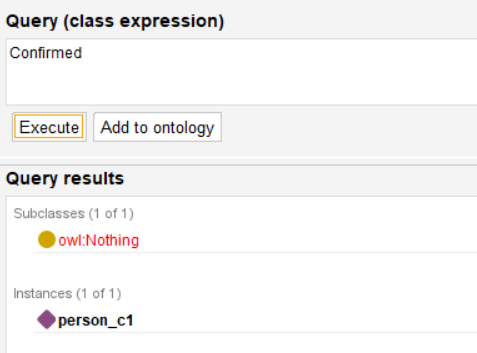
\includegraphics[width=0.7\textwidth]{an1.png}
	\caption{Consulta no Protégé para verificar a classificação de \texttt{person\_c1}}
	\label{fig:an1}
\end{figure}

Clicando na aba \textit{Classes} consultou-se a definição de \texttt{Confirmed} que era a seguinte:

\begin{center}
	\begin{verbatim}
		hasTestOutcomeOf some ({SARS-CoV-2-positive})
	\end{verbatim}
\end{center}

Para construir o \textit{tableau} consultou-se os slides do professor \cite[pág. 30]{Trigo_2025}.

Para verificar se uma instância é verdade, temos de negar esse conceito e verificar se existe \textit{clash}. Caso exista, o conceito é satisfeito.

Seguindo a ideia descrita acima fez-se a seguinte elaboração:

\[
\mathit{Confirmed} \equiv \exists\,\text{hasTestedOutcomeOf}.\text{SARS-CoV-2-positive}
\]

\[
\big(\mathcal{A} \models \text{Confirmed}(\text{person\_c1})\big)
\Leftrightarrow
\mathcal{A} \cup \{\neg\text{Confirmed}(\text{person\_c1})\}
\ \text{não-satisfeito em } \mathcal{T}
\]

\begin{figure}[htbp]
	\centering
	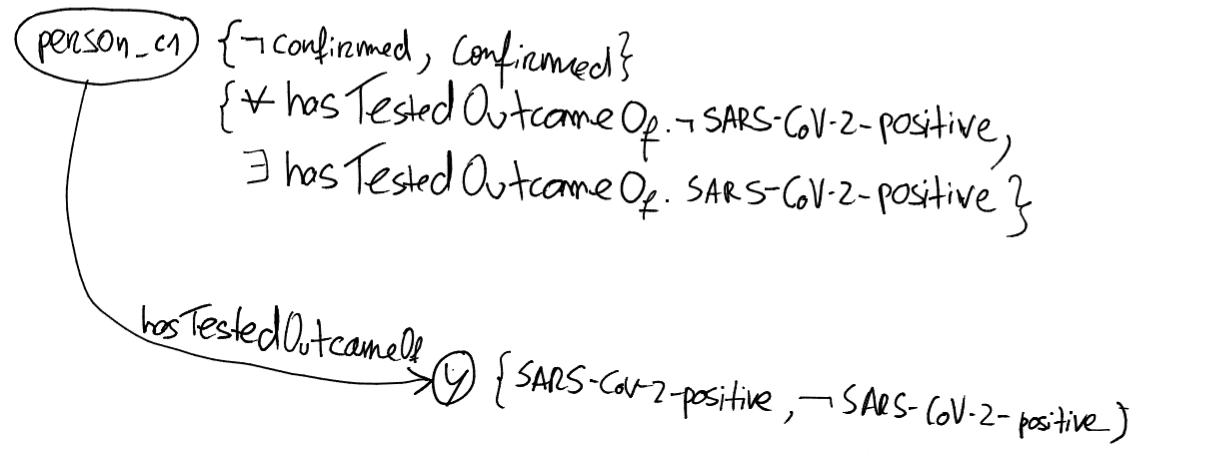
\includegraphics[width=0.7\textwidth]{an2.png}
	\caption{\textit{Tableau} para demonstrar classificação de \texttt{person\_c1}}
	\label{fig:an2}
\end{figure}

O Conceito é satisfeito, pois a negação de
$\text{Confirmed}(\text{person\_c1})$ não foi satisfeita, devido ao \textit{clash} presente na figura acima.
%%________________________________________________________________________
\chapter{Definir Relações}
\label{ch:defRel}
%%________________________________________________________________________

Neste ponto, tinha de se definir relações para que \texttt{person\_p2} fosse classificado como \textit{Probable}.

Ao consultar \texttt{person\_p2} no Protégé, verificou-se que este não tinha qualquer relação ou outro tipo de informação atribuída.

Desta forma, foi necessário fazer todas relações necessárias. E optou-se por adicionar \texttt{hasTestOutcomeOf SARS-CoV-2-not-conclusive} e \texttt{isExplainedBy \_none\_}. Isto, porque a definição de \textit{Probable} é: 

\begin{center}
	\begin{verbatim}
		((hasTestOutcomeOf value SARS-CoV-2-not-conclusive) or
		 (hasTestOutcomeOf value pan-coronavirus-positive))
		and (isExplainedBy value _none_)
	\end{verbatim}
\end{center}

Passando para uma expressão de Lógica de Descrição:

\begin{align*}
	\mathit{Probable} \equiv 
	& \Big(\exists\,\text{hasTestOutcomeOf}.\{\text{SARS-CoV-2-non-conclusive}\} \\
	& \quad \sqcup\ \exists\,\text{hasTestedOutcomeOf}.\{\text{pan-coronavirus-positive}\}\Big) \\
	& \quad \sqcap \exists\,\text{isExplainedBy}.\{\text{none}\}
\end{align*}

Também se demonstrou com a ajuda do \textit{tabelau} a classificação de \texttt{person\_p2}.

\begin{figure}[htbp]
	\centering
	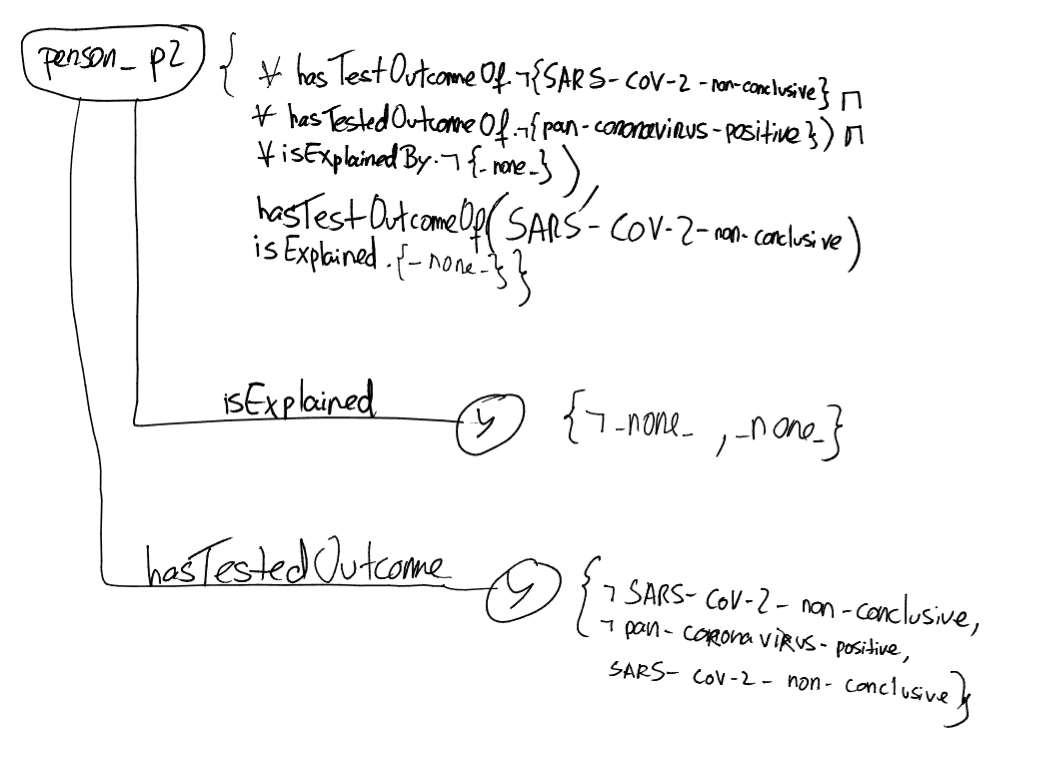
\includegraphics[width=0.7\textwidth]{an3.png}
	\caption{\textit{Tableau} para demonstrar classificação de \texttt{person\_p2}}
	\label{fig:an3}
\end{figure}

O conceito é satisfeito, pois a negação de
$\text{Probable}(\text{person\_p2})$ não foi satisfeita, devido ao \textit{clash} presente na figura acima.

Já no Protégé o resultado também foi satisfatório como demonstra a imagem recortada abaixo:

\begin{figure}[htbp]
	\centering
	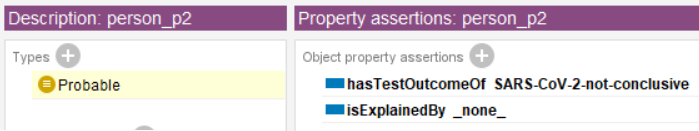
\includegraphics[scale=0.9]{an4.png}
	\caption{Resultados da classificação de \texttt{person\_p2} no Protégé}
	\label{fig:an4}
\end{figure}

%%________________________________________________________________________
\chapter{Definir conceito de \textit{Suspicious}}
\label{ch:sus}
%%________________________________________________________________________

Nesta alínea era preciso definir o conceito para o caso \textit{Suspicious}, tendo por base o documento oficial da DGS.

Realizou-se o seguinte raciocínio:

\textbf{Caso Suspeito}

\noindent $1$ - Infeção Respiratória (IR):
\[
\big(\text{IR} \sqcap (\text{VTA} \sqcup \text{RTA}) \sqcap E\{\text{none}\} \sqcap St\{14\}\big)
\]
(Viagem ($\text{VTA}$) ou Residência ($\text{RTA}$) com transmissão ativa, sem etiologia ($\text{E}$),
sintomas ($\text{St}$) c/14 dias)

\noindent $2$ - IR:
\[
\big(\text{IR} \sqcap (\text{CC}(\text{Cf} \sqcup \text{Prv}))\big) \sqcap St\{14\}
\]
(Contacto ($\text{CC}$) com caso confirmado ($\text{Cf}$) ou provável ($\text{Prv}$) de
SARS-CoV-2 ou COVID-19, sintomas c/14 dias)

\noindent $3$ - IR:
\[
\big(\text{IR} \sqcap M\{grh\} \sqcap E\{\text{none}\}\big)
\]
(Manifesta IR ($M$) grave, requer hospitalização ($\{grh\}$), sem etiologia)

\noindent obs: \textit{``grh''} é indivíduo de $\text{IR}$, \textit{logo} $M\{\text{IR}\}$.

Depois estas conclusões foram traduzidas para o Protégé da seguinte forma:

\begin{center}
	\begin{verbatim}
		(AcuteRespiratoryInfection
		and ((hasResidenceIn some AreaWithActiveCommunityTransmission) or 
		(hasTraveledFrom some AreaWithActiveCommunityTransmission))
		and (hasSymptomsStartingSince value _014-days-ago)
		and (isExplainedBy value _none_)) or
		(AcuteRespiratoryInfection
		and (hasContactWith some (Confirmed or Probable))
		and (hasSymptomsStartingSince value _014-days-ago)) or
		((hasManifestationOf some AcuteRespiratoryInfection)
		and (isExplainedBy value _none_))
	\end{verbatim}
\end{center}

%%________________________________________________________________________
\chapter{Verificações e trabalho no Protégé}
\label{ch:prot}
%%________________________________________________________________________

Na última parte do trabalho começou-se por verificar se \texttt{person\_s1} e \texttt{person\_s2} são corretamente classificadas como \textit{Suspicious}.

O \texttt{person\_s1} foi bem classificado logo de primeiro, mas o \texttt{person\_s2} teve de ter uma relação acrescentada: \texttt{isExplainedBy{\_none\_}}.

Desta forma, ambos os indivíduos ficaram bem classificados.

Depois, tinha-se de definir as relações necessárias para que \texttt{person\_s3} seja classificada como \texttt{Suspicious}. Como este indivíduo já tinha definido um tipo (\texttt{hasManifestationOf some AcuteRespiratoryInfection}), foi apenas preciso adicionar \texttt{isExplainedBy \_none\_}, tal qual na alínea anterior.

Por último, tinha-se de definir as relações necessárias para que \texttt{person\_s4} seja classificada como \texttt{Suspicious} e que estivesse em contacto com \texttt{person\_s2}.

Tal como no caso da \texttt{person\_s3}, foi necessário adicionar a relação \texttt{is ExplainedBy \_none\_} e, para representar a situação de contacto com \texttt{person \_s2}, também adicionou-se a relação \texttt{hasContactWith person\_s2}.